\begin{figure}[H]
\centering
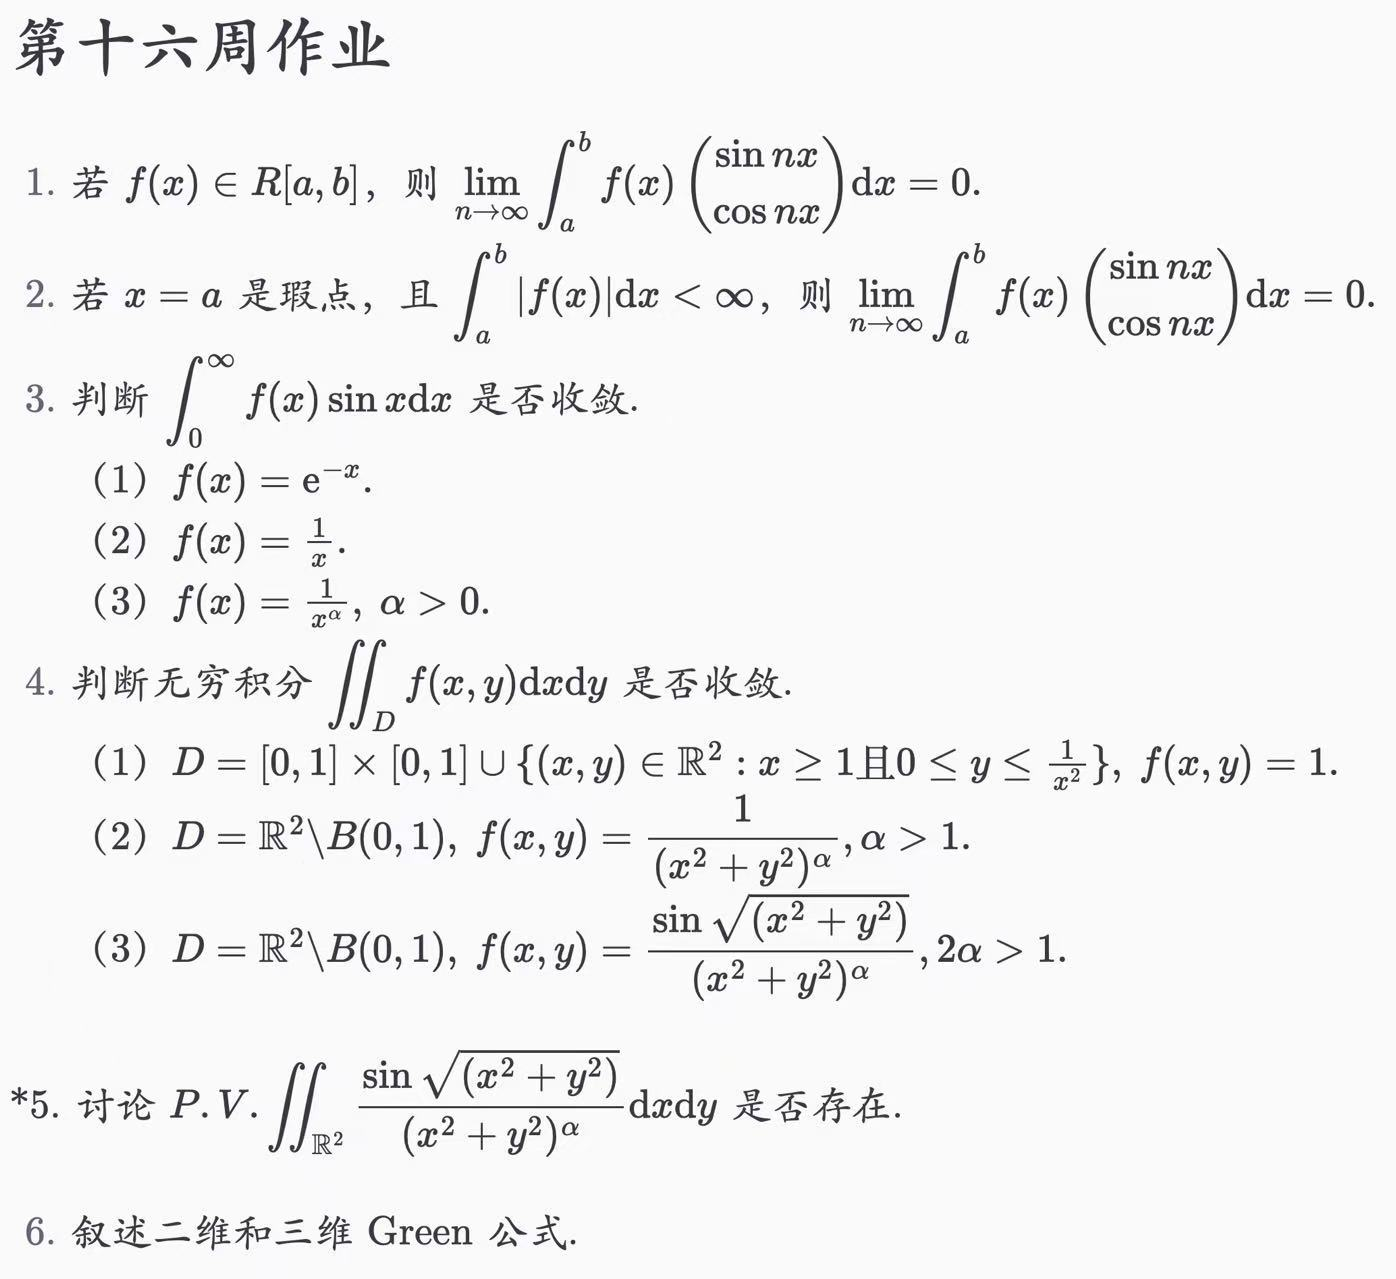
\includegraphics[width=\textwidth]{9e859e5d2baf3a0b21052046cfca336f.jpg}
% \caption{}
\label{}
\end{figure}

\begin{exercise}
若 $f(x) \in R[a, b]$, 则 $\lim _{n \rightarrow \infty} \int_a^b f(x)\binom{\sin n x}{\cos n x} \mathrm{~d} x=0$.
\end{exercise}
\begin{proof}
对任意 $\epsilon>0$,存在划分 $P=\{ x_0=a,x_1,\dots,x_r=b \}$ 使得
\[
\sum_{k=1}^{r} (M_k-m_k)\Delta x_k\leq \frac{\epsilon}{2}
\]
于是
\[
\begin{aligned}
\left\lvert  \int_{a}^{b} f(x)\sin (nx) \, \mathrm{d}x   \right\rvert  & =\left\lvert  \sum_{k=1}^{r} \int_{x_{k-1}}^{x_k} (f(x)-m_k)\sin (nx) \, \mathrm{d}x +\sum_{k=1}^{r} \underbrace{ \int_{x_{k-1}}^{x_k} m_k\sin (nx) \, \mathrm{d}x }_{ =\frac{m_k}{n}(\cos(nx_{k-1})-\cos(nx_k))   }    \right\rvert \\
 & \leq \sum_{k=1}^{r} \int_{x_{k-1}}^{x_k} \lvert f(x)-m_k \rvert \cdot \lvert \sin(nx) \rvert   \, \mathrm{d}x +\frac{2}{n}\cdot\sum_{k=1}^{r} \lvert m_k \rvert   \\
 & \leq \sum_{k=1}^{r} (M_k-m_k)\Delta x_k+\frac{2}{n}\cdot\sum_{k=1}^{r} \lvert m_k \rvert \\
 & \leq \frac{\epsilon}{2}+\frac{2}{n}\cdot\sum_{k=1}^{r} \lvert m_k \rvert
\end{aligned}
\]
取 $n\geq\frac{\epsilon}{4K}$ 其中 $K\coloneqq \sum_{k=1}^{r}\lvert m_k \rvert$,就有 $\left\lvert  \int_{a}^{b} f(x)\sin(nx) \, \mathrm{d}x  \right\rvert\leq\epsilon$. 于是
\[
\lim_{ n \to \infty } \int_{a}^{b} f(x)\sin(nx) \, \mathrm{d}x =0
\]
同理
\[
\lim_{ n \to \infty } \int_{a}^{b} f(x)\cos(nx) \, \mathrm{d}x =0
\]
于是
\[
\lim _{n \rightarrow \infty} \int_a^b f(x)\binom{\sin n x}{\cos n x} \mathrm{~d} x=0
\]
\end{proof}

\begin{exercise}
若 $x=a$ 是瑕点,且 $\int_a^b|f(x)| \mathrm{d} x<\infty$ ,则 $\lim _{n \rightarrow \infty} \int_a^b f(x)\binom{\sin n x}{\cos n x} \mathrm{~d} x=0$ .
\end{exercise}
\begin{proof}
不妨设 $f$ 只有一个瑕点 $a$, 于是对于任意给定的 $\epsilon>0$,存在充分小的 $\delta>0$,使得
\[
\left\lvert  \int_{a}^{a+\delta} f(x)\sin(nx) \, \mathrm{d}x   \right\rvert \leq \int_{a}^{a+\delta} \lvert f(x) \rvert  \, \mathrm{d}x\leq \frac{\epsilon}{2}
\]
同时 $f$ 在 $[a+\delta,b]$ 上黎曼可积,于是存在充分大的 $N$,使得当 $n>N$ 时
\[
\left\lvert  \int_{a+\delta}^{b} f(x)\sin(nx) \, \mathrm{d}x  \right\rvert \leq \frac{\epsilon}{2}
\]
于是
\[
\left\lvert  \int_{a}^{b} f(x)\sin(nx) \, \mathrm{d}x   \right\rvert \leq \left\lvert  \int_{a}^{a+\delta} f(x)\sin(nx) \, \mathrm{d}x   \right\rvert +\left\lvert  \int_{a+\delta}^{b} f(x)\sin(nx) \, \mathrm{d}x   \right\rvert \leq \epsilon
\]
于是
\[
\lim_{ n \to \infty } \int_{a}^{b} f(x)\sin(nx) \, \mathrm{d}x =0
\]
同理
\[
\lim_{ n \to \infty } \int_{a}^{b} f(x)\cos(nx) \, \mathrm{d}x =0
\]
于是
\[
\lim _{n \rightarrow \infty} \int_a^b f(x)\binom{\sin n x}{\cos n x} \mathrm{~d} x=0
\]
\end{proof}

\begin{exercise}
判断 $\int_0^{\infty} f(x) \sin x \mathrm{~d} x$ 是否收敛.
	\begin{enumerate}
		\item $f(x)=\mathrm{e}^{-x}$ .
		\item $f(x)=\frac{1}{x}$ .
		\item $f(x)=\frac{1}{x^\alpha}, \alpha>0$ .
	\end{enumerate}
\end{exercise}
\begin{proof}
由 Dirichlet 判别法,$\left\lvert  \int_{0}^{N} \sin x \, \mathrm{d}x  \right\rvert\leq2$ 有界,三个 $f(x)$ 都单调递减趋于 0,故广义积分 $\int_{0}^{\infty} f(x)\sin x \, \mathrm{d}x$ 收敛.
\end{proof}

\begin{exercise}
判断无穷积分 $\iint_D f(x, y) \mathrm{d} x \mathrm{~d} y$ 是否收敛.
	\begin{enumerate}
		\item $D=[0,1] \times[0,1] \cup\left\{(x, y) \in \mathbb{R}^2: x \geq 1\right.$ 且 $\left.0 \leq y \leq \frac{1}{x^2}\right\}, f(x, y)=1$ .
		\item $D=\mathbb{R}^2 \backslash B(0,1), f(x, y)=\frac{1}{\left(x^2+y^2\right)^\alpha}, \alpha>1$ .
		\item $D=\mathbb{R}^2 \backslash B(0,1), f(x, y)=\frac{\sin \sqrt{\left(x^2+y^2\right)}}{\left(x^2+y^2\right)^\alpha}, 2 \alpha>1$ .
	\end{enumerate}
\end{exercise}
(1)
\[
\begin{aligned}
\iint_{D}f(x,y)\mathrm{d}x\mathrm{d}y & =\iint_{[0,1]^{2}} 1 \mathrm{d}x\mathrm{d}y+\lim_{ N \to \infty } \int_{1}^{N} \int_{0}^{x^{-2}} 1 \, \mathrm{d}y  \, \mathrm{d}x  \\
 & =1+\lim_{ N \to \infty } \int_{1}^{N} x^{-2} \, \mathrm{d}x  \\
 & =1+\lim_{ N \to \infty }(1-N^{-1}) \\
 & =2
\end{aligned}
\]
收敛.

(2) 定义见汪林:
\begin{figure}[H]
\centering
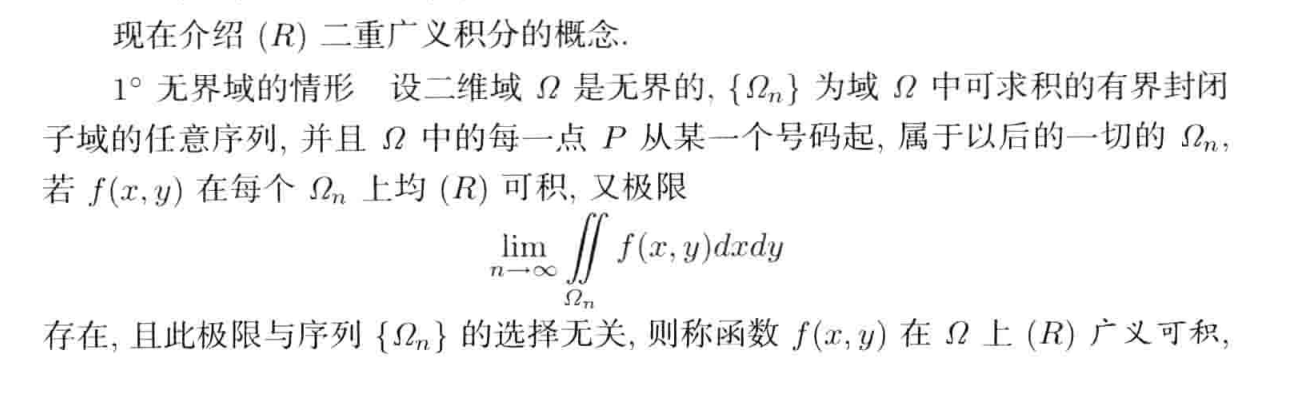
\includegraphics[width=\textwidth]{hw15-2025061317.png}
% \caption{}
\label{}
\end{figure}
\begin{figure}[H]
\centering

\includegraphics[width=\textwidth]{1-hw15-2025061317.png}
% \caption{}
\label{}
\end{figure}

对于任意 $R>1$,
\[
\iint_{B_{R}(0)\setminus B_1(0)}\lvert f(x,y) \rvert \mathrm{d}x\mathrm{d}y=\int_{1}^{R} \int_{0}^{2\pi} \frac{1}{r^{2\alpha}} \, \mathrm{d}\theta  \, \mathrm{d}r=\frac{\pi}{\alpha-1}(1-R^{2-2\alpha})  
\]
根据二重无穷积分的定义
\[
\iint_{D}\lvert f(x,y) \rvert \mathrm{d}x\mathrm{d}y=\lim_{ R \to \infty } \iint_{B_{R}(0)\setminus B_1(0)}\lvert f(x,y) \rvert \mathrm{d}x\mathrm{d}y=\frac{\pi}{\alpha-1}
\]
$f$ 绝对收敛,$f$ 非负,故无穷积分 $\iint_D f(x, y) \mathrm{d} x \mathrm{~d} y$ 收敛.

(3)
这应该是个广义黎曼积分吧. 那简单讨论(结合 Fubini 定理,广义二重黎曼积分定义)就可以保证
\[
\iint_{D}f(x,y)\mathrm{d}x\mathrm{d}y=\lim_{ R \to \infty } \int_{0}^{2\pi} \int_{1}^{R} \frac{\sin r}{r^{2\alpha-1}} \, \mathrm{d}r  \, \mathrm{d}\theta=\lim_{ R \to \infty } 2\pi \int_{1}^{R} \frac{\sin r}{r^{2\alpha-1}} \, \mathrm{d}r
\]
其中 $\left\lvert  \int_{1}^{R} \sin r \, \mathrm{d}r  \right\rvert\leq2$ 有界,$\frac{1}{r^{2\alpha-1}}$ 单调递减趋于 0,由 Dirichlet 判别法,上述积分收敛.

\begin{exercise}
讨论 P.V. $\iint_{\mathbb{R}^2} \frac{\sin \sqrt{\left(x^2+y^2\right)}}{\left(x^2+y^2\right)^\alpha} \mathrm{d} x \mathrm{~d} y$ 是否存在.
\end{exercise}
当且仅当 $2\alpha>1$ 时,$\iint_{D}\frac{\sin \sqrt{ x^{2}+y^{2} }}{(x^{2}+y^{2})^{\alpha}}\mathrm{d}x\mathrm{d}y$ 存在,其中 $D=\mathbb{R}^{2}\setminus B_1(0)$. 只需要看极限
\[
\lim_{ \epsilon \to 0^{+} } \iint_{B_1(0)\setminus B_{\epsilon}(0)}\frac{\sin \sqrt{ x^{2}+y^{2} }}{(x^{2}+y^{2})^{\alpha}}\mathrm{d}x\mathrm{d}y
\]
是否存在.
\[
 \iint_{B_1(0)\setminus B_{\epsilon}(0)}\frac{\sin \sqrt{ x^{2}+y^{2} }}{(x^{2}+y^{2})^{\alpha}}\mathrm{d}x\mathrm{d}y=\int_{0}^{2\pi} \int_{\epsilon}^{1} \frac{\sin r}{r^{2\alpha-1}} \, \mathrm{d}r  \, \mathrm{d}\theta=2\pi \int_{\epsilon}^{1} \frac{\sin r}{r^{2\alpha-1}} \, \mathrm{d}r  
\]
$\frac{\sin r}{r^{2\alpha-1}}\sim r^{2-2\alpha}$ as $r\to0$, 于是上述积分存在当且仅当 $2-2\alpha>-1$,也就是 $\alpha<\frac{3}{2}$. 于是当且仅当 $\frac{1}{2}<\alpha<\frac{3}{2}$ 时,P.V. $\iint_{\mathbb{R}^2} \frac{\sin \sqrt{\left(x^2+y^2\right)}}{\left(x^2+y^2\right)^\alpha} \mathrm{d} x \mathrm{~d} y$ 存在.

\begin{exercise}
叙述二维和三维 Green 公式.
\end{exercise}
在二维空间中,设 $D$ 是平面上的单连通区域,其边界 $\partial D$ 是分段光滑的简单闭曲线,方向为正(即沿边界行走时区域 $D$ 始终在左侧)。设 $P(x, y)$ 和 $Q(x, y)$ 是定义在包含 $D$ 及其边界的开区域上的连续可微函数,则有
\[
\oint_{\partial D} P \, dx + Q \, dy = \iint_D \left( \frac{\partial Q}{\partial x} - \frac{\partial P}{\partial y} \right) \, dA.
\]
在三维空间中(高斯公式或散度定理),设 $V$ 是 $\mathbb{R}^3$ 中的有界闭区域,其边界 $\partial V = S$ 是分段光滑的闭合曲面,取外侧法向量。设向量场 $\mathbf{F}(x, y, z) = P(x, y, z) \mathbf{i} + Q(x, y, z) \mathbf{j} + R(x, y, z) \mathbf{k}$ 是在包含 $V$ 及其边界的开区域上连续可微的,则有
\[
\iint_S \mathbf{F} \cdot \mathbf{n} \, dS = \iiint_V \nabla \cdot \mathbf{F} \, dV,
\]
或写成分量形式
\[
\iint_S (P \cos \alpha + Q \cos \beta + R \cos \gamma) \, dS = \iiint_V \left( \frac{\partial P}{\partial x} + \frac{\partial Q}{\partial y} + \frac{\partial R}{\partial z} \right) \, dV,
\]
其中 $(\cos \alpha, \cos \beta, \cos \gamma)$ 是曲面 $S$ 的单位外法向量的方向余弦。
